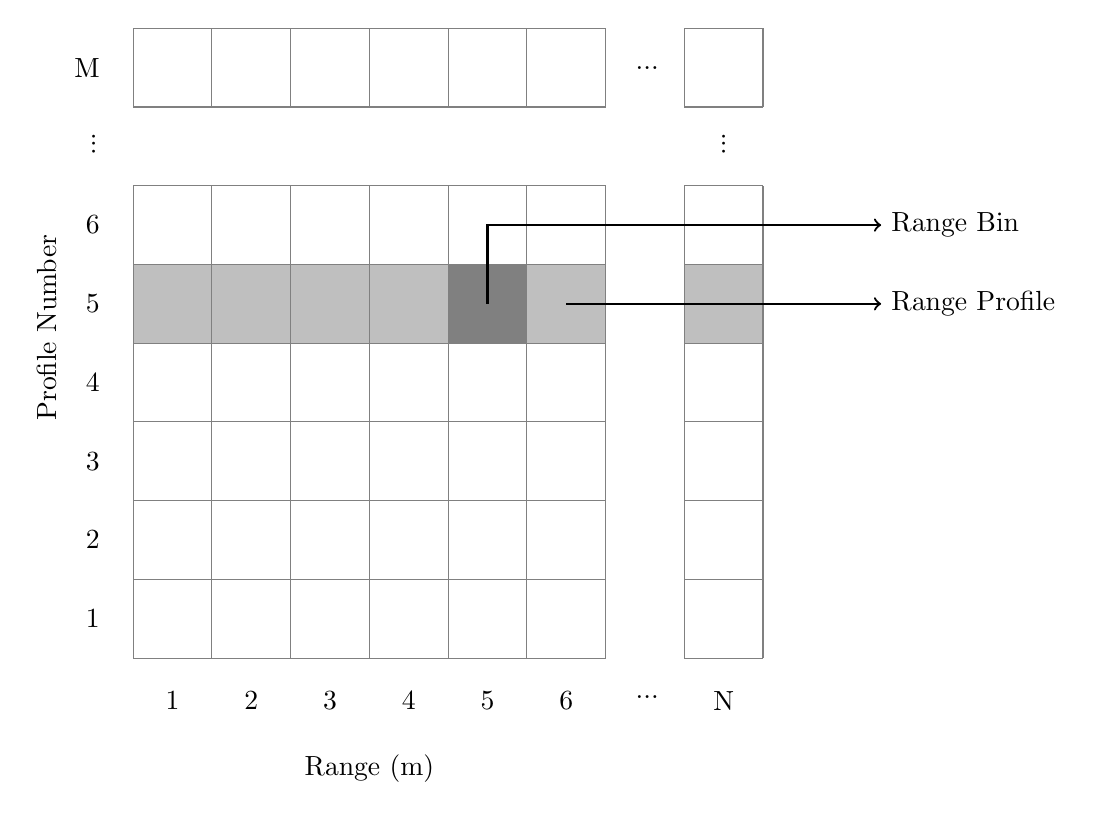
\begin{tikzpicture}

% Draw grid
\draw[step=1cm,black!50,thin] (0,0) grid (6,6);

\draw[step=1cm,black!50,thin] (7,0) grid (8,6);
\draw[step=1cm,black!50,thin] (7,7) grid (8,8);
\draw[step=1cm,black!50,thin] (0,7) grid (6,8);


\foreach \x in {1,...,6}
  \node[below] at (\x-0.5,-0.3) {\x};

% Add numbers to the y-axis of the first grid (centered between cells)
\foreach \y in {1,...,6}
  \node[left] at (-0.3,\y-0.5) {\y};

% Label the axes of the first grid (centered between cells)
\node[below=0.8cm] at (3,-0.3) {Range (m)};
\node[left=0.8cm,rotate=90] at (-0.3,5.5) {Profile Number};

% % Fill the row with white
% \fill[white] (0,7) rectangle (6,6);

% Add a row above the second grid with the y-axis label "N"
\node[left, rotate = 90] at (-0.5,6.8) {...};
\node[left] at (-0.3,7.5) {M};
\node[left, rotate = 90] at (7.5,6.8) {...};
\node[left] at (6.8,-0.5) {...};
\node[left] at (6.8,7.5) {...};
\node[below] at (7.5, -0.3) {N};

% Fill the entire fourth row of the first grid with transparent gray
\fill[gray, opacity=0.5] (0,4) rectangle (6,5);
\fill[gray, opacity=0.5] (7,4) rectangle (8,5);

% Fill the last cell in the fourth row of the first grid with gray
\fill[gray, opacity=1] (4,4) rectangle ++(1,1);

% Add an arrow and label "range profile"
\draw[->, thick] (5.5,4.5) -- (9.5,4.5) node[right] {Range Profile};
% Add an arrow and label "range bin" pointing to the side
\draw[->, thick] (4.5,4.5) -- (4.5,5.5) -- (9.5,5.5) node[right] {Range Bin};

\end{tikzpicture}